\subsection{Результат внедрения}\label{subsec:results}

В рамках данной работы структура данных Сито-индекс была внедрена~\cite{Sieve_Github} в платформу для доступа к данным Apache Hudi.

В данном разделе представлены результаты сравнения скорости работы точечных и интервальных запросов с использованием упрощенных сводок и Сито-индекса для таблиц разного размера. Тестовый набор данных был сгенерирован с использованием специализированной библиотеки примеров для больших данных TPC-H~\cite{TPC-H}, запросы производились к таблице {<<lineitem>>} по атрибуту {<<shipdate>>}.

В процессе тестирования индекс был построен для двух таблиц разного размера: первые 20 миллионов строк (первый набор данных) и первые 600 миллионов строк (второй набор данных) из таблицы {<<lineitem>>}. Тестовый вычислительный кластер Spark состоял из одного узла, который был ограничен объемом оперативной памяти в 2 ГБ. Это позволило проверить возможность индексации таблицы из 20 миллионов записей с полной загрузкой всех значений атрибута в память и возможность построения индекса для таблицы из 600 миллионов записей, размер индексируемого атрибута такой таблицы не умещается в 2 ГБ оперативной памяти.

Размер индекса для первого набора данных составил 1,5 МБ при общем размере индексируемого атрибута в 80 МБ (20 миллионов значений по 4 Б), а для второго — 52 МБ при общем размере индексируемого атрибута 2,2 ГБ (600 миллионов значений по 4 Б) (Рисунок \ref{figure:index_size}). При этом размер индекса составил примерно $6\%$ от исходного размера индексируемого атрибута.

\begin{figure}[h]
    \centering
    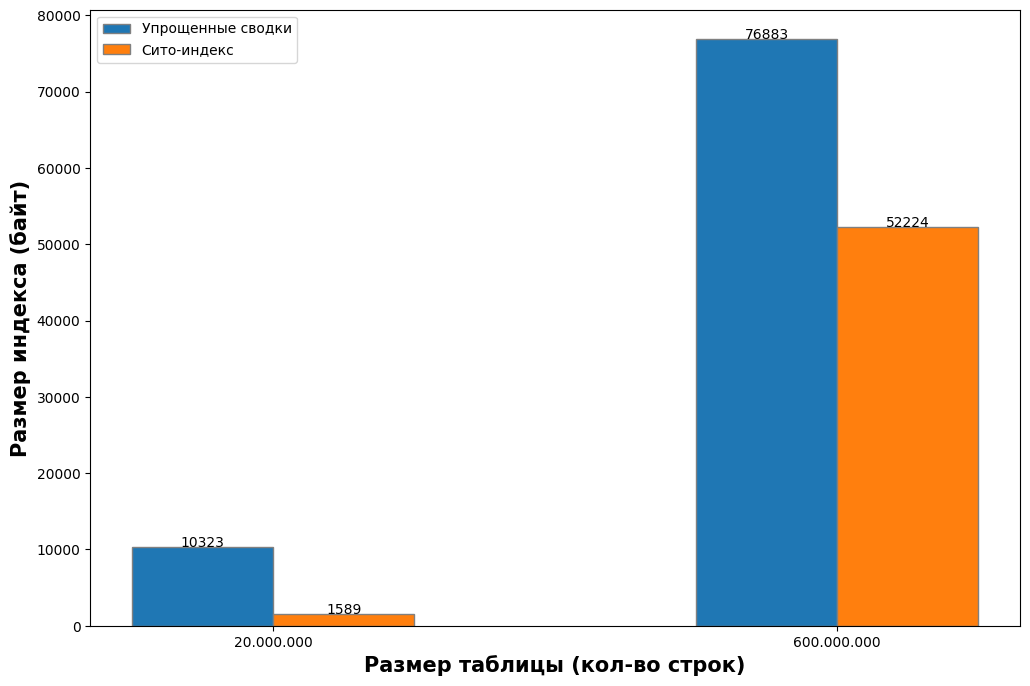
\includegraphics[scale=0.56]{4_index_size.png}
    \caption{\centering{Итоговые размера упрощенных сводок и Сито-индекса на файловой системе для двух таблиц разного размера}}
    \label{figure:index_size}
\end{figure}

Причина, по которой итоговый размер упрощенных сводок получился больше размера Сито-индекса заключается в реализации упрощенных сводок в Apache Hudi~\cite{Hudi_MetadataPayload}, каждая запись содержит полное название файловой группы (Определение \ref{def:location}), в то время как авторская реализация Сито-индекса кодирует каждый идентификатор файловой группы используя ассоциативный массив, что позволяет сократить использование памяти. 

Далее была проведены серии из 50 точечных запросов и 20 интервальных запросов для двух наборов данных, сперва они были проиндексированы упрощенными сводками, затем Сито-индексом. На рисунках ниже представлено сравнение средней скорости выполнения точечных (Рисунок \ref{figure:point_query}) и интервальных (Рисунок \ref{figure:range_query}) запросов. Разброс значений в сериях запросов составил не более 3\%.

\begin{figure}[h]
    \centering
    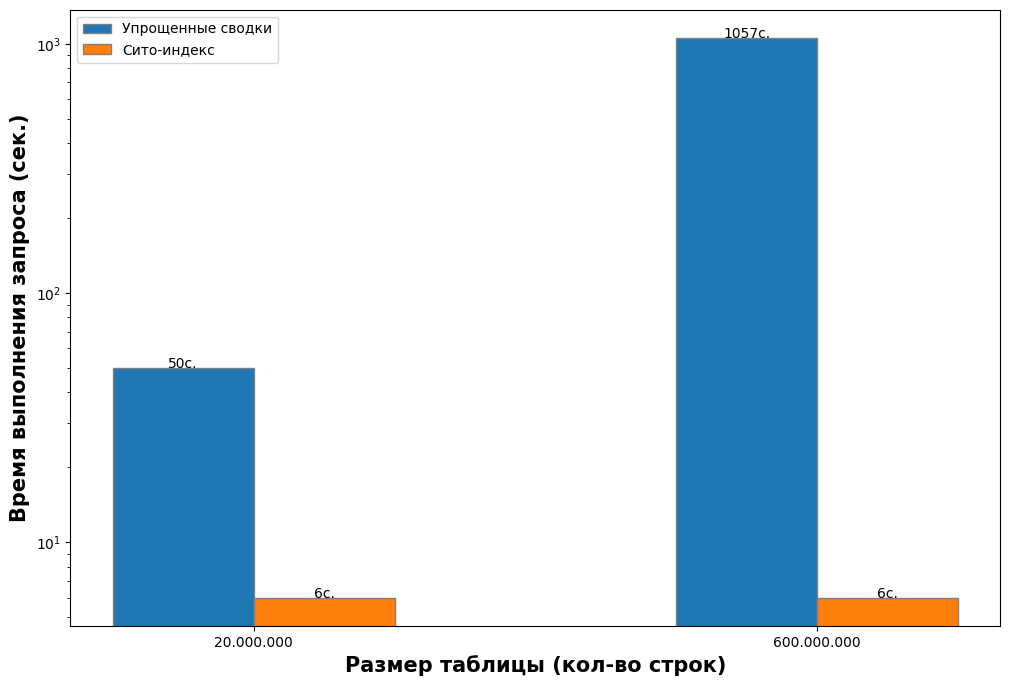
\includegraphics[scale=0.62]{1_point_query.png}
    \caption{\centering{Среднее время выполнения точечного запроса с использованием упрощенных сводок и Сито-индекса для двух таблиц разного размера}}
    \label{figure:point_query}
\end{figure}


\begin{figure}[h]
    \centering
    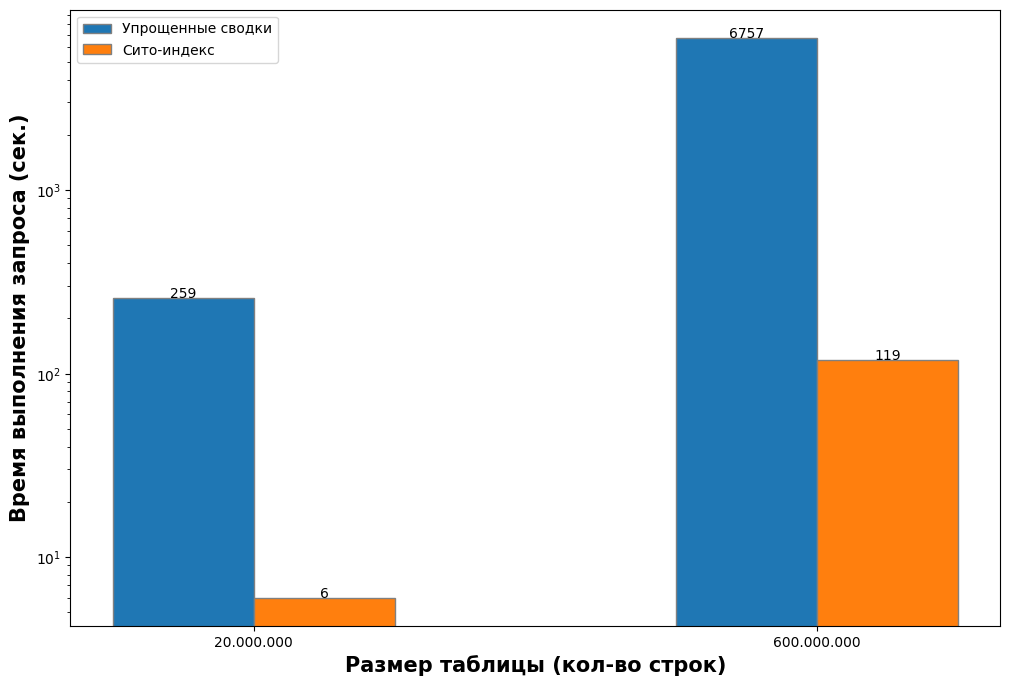
\includegraphics[scale=0.62]{2_range_query.png}
    \caption{\centering{Среднее время выполнения интервального запроса с использованием упрощенных сводок и Сито-индекса для двух таблиц разного размера}}
    \label{figure:range_query}
\end{figure}

В наиболее выигрышном для Сито-индекса случае, почти каждый файл с данными в обеих наборах содержал минимальное значение даты --- 1 января 1992 года, а максимальное --- 1 января 2008 года, при этом почти каждый файл сдержал каждую дату из интервала с 1 января 1992 года по 1 января 1998 года и каждую дату из интервала с 1 января 2007 года по 1 января 2008 года, промежуток с 1999 года по 2006 год оставался пустым. Интервальные запросы были выполнены с предикатом $1$ января $2003$г. $\leq shipdate \leq 31$ января $2003$г., а точечные с предикатом $shipdate = 1$ января $2003$г. Тогда индекс с упрощенными сводками приводил к чтению всех файлов, а Сито-индекс пропускал чтение почти всех файлов.

В наименее выигрышном для Сито-индекса случае, когда выполнения запросов с предикатом подразумевало чтение всех файлов, время выполнения запроса было одинаковым для Сито-индекса и упрощенных сводок.

Построение Сито-индекса занимает больше времени ввиду большей вычислительной сложности алгоритма построения индекса. Однако является сопоставимым с построением упрощенных сводок, так как для построения упрощенных сводок необходимо прочитать весь индексируемый атрибут, в то время как для построения Сито-индекса его необходимо еще и отсортировать.

Далее представлено сравнение времени построения индекса для двух наборов данных (Рисунок \ref{figure:index_build_time}).

\begin{figure}[h]
    \centering
    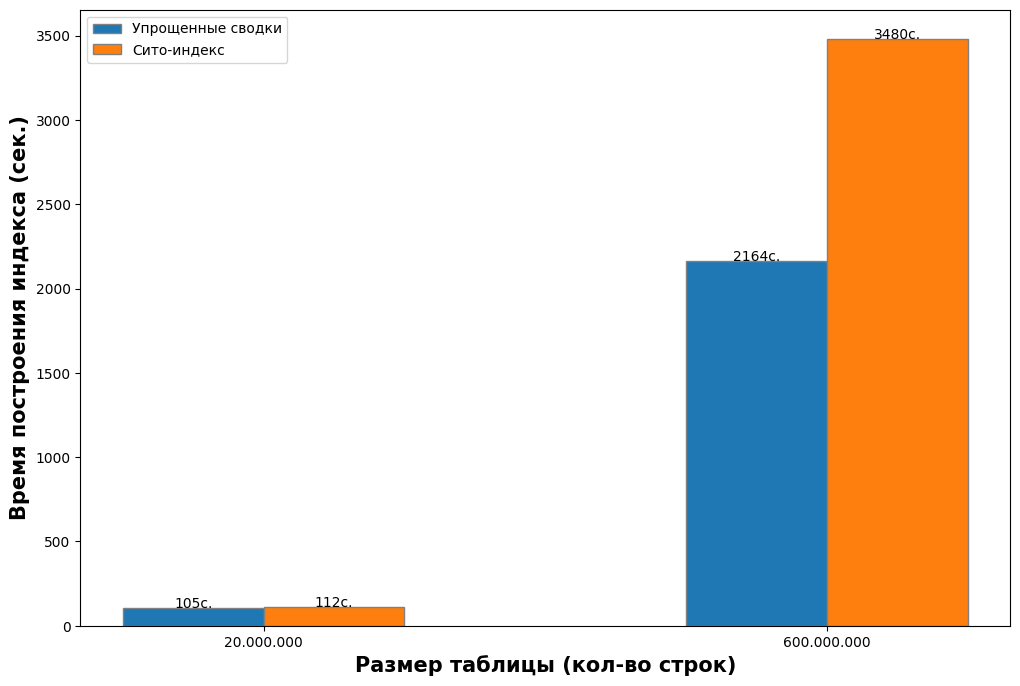
\includegraphics[scale=0.62]{3_build_time.png}
    \caption{\centering{Сравнение времени построения упрощенных сводок и Сито-индекса для двух таблицах разного размера}}
    \label{figure:index_build_time}
\end{figure}

\newpage
\section*{Выводы}
\addcontentsline{toc}{section}{Выводы}

Благодаря разработке структуры данных Сито-индекс, которая построена на основе структуры данных Sieve и является ее модернизацией, и внедрению ее в систему для доступа к данным с открытым исходным кодом Apache Hudi, удалось добиться прироста скорости выполнения точечных запросов на порядки, а интервальных запросов на порядок для тех сценариев использования, когда имеющиеся в Apache Hudi фильтры для отсеивания нерелевантных файлов упрощенные сводки были не способны отсеивать файлы.

В худших же сценариях для использования Сито-индекса время выполнения запросов с данной структурой было не больше времени выполнения тех же запросов с использованием упрощенных сводок.
